\documentclass[review]{elsarticle}

\usepackage{amssymb}
%% The amsthm package provides extended theorem environments
\usepackage{amsthm}
\usepackage{amsmath}
\usepackage{float}
\usepackage{bm}
\usepackage{subfigure}
\usepackage{tikz}
\usetikzlibrary{shapes,arrows}
\usepackage{lineno,hyperref}
\modulolinenumbers[5]

\journal{Journal of \LaTeX\ Templates}

%%%%%%%%%%%%%%%%%%%%%%%
%% Elsevier bibliography styles
%%%%%%%%%%%%%%%%%%%%%%%
%% To change the style, put a % in front of the second line of the current style and
%% remove the % from the second line of the style you would like to use.
%%%%%%%%%%%%%%%%%%%%%%%


%\begin{enumerate}
%\item[a] Our work builds on a currently available meam potential from CPL 2010. We managed to put meam parameters from the paper into lammps, which have the data format:
%\begin{equation*}
%\begin{aligned}
%&\text{pair\_style    meam} \\
%&\text{pair\_coeff    * * library.meam Si4 Ge5  SiGe.meam Si4 Ge5}
%\end{aligned}
%\end{equation*}
%{\color{red} A mistake in the previous SiGe.meam. In the first line, Ec(1,2) should be equal to 4.23. Sorry about that.}
%
%\item[b] We also found several issues in the CPL 2010 paper, 1) they have some correction functions to modify the radial distribution function of the liquid alloy, which is not implemented in LAMMPS,  which should not have significant effects on simulations of solid devices. 
%2) They made mistakes in the parameter table in the r\_e column. 
%3) The elastic constants for SiGe can be extracted from the following figures, as listed below:
%C11 = 181.03 GPa, C12 = 80.57 GPa, and C44 = 85.36 GPa, which quantitatively agree with experimental measured values.
%4) In the paper, they claim that they fit the lattice constant of SiGe to 5.5285 A, to match the experimental value. But actually the experiential value is  5.5377 A. 
%5) How they obtained the lattice constant curve in the paper is not clearly stated. However, from the results, one can infer that Firstly, the data should be obtained from finite temperature simulations, because otherwise the lattice constant of Si is not 5.431 A. Then  curves are shifted to match the lattice constant of Si with experimental value. 
%
%\item[c] An important parameter for our study is the equilibrium lattice constant of $Si_{1-x}Ge_x$. The lattice constant can be approximated as a function the compositions as
%\begin{equation*}\label{eq:analy_lattice}
%\text{Lattice constant } a(x) \text{ of } Si_{1-x}Ge_x = ( 5.431 + 0.20x + 0.027x^2) A \text{ at } 300 K
%\end{equation*}
%(http://www.ioffe.ru/SVA/NSM/Semicond/SiGe/basic.html).
%As a benchmark test for this property, we created a large Si crystal and randomly replace Si atoms with Ge atoms. The simulation is performed with free box. Then the volume is computed to predicted the lattice constants at equilibrium.
%
%We managed to get the values of the lattice constants for different Ge compositions at both 0K and 300K. As shown in Fig. \ref{fig:latt_xGe}, the lattice constants are compared from simulation (0K relaxation), Vegard's law and experimental data, with Eqn. \ref{eq:analy_lattice}. It is observed that the simulation data slightly deviate from the Vegard's. While most of the data are close to the experimental values,  the lattice constant is underestimated when Ge composition is around $0.5$.
%
%Figure \ref{fig:cpl_lattice} is shown below, in which the same comparison, which shows that our data is consistent with the CPL 2010 paper. 
%Figure \ref{fig:yanming_lattice} shows the lattice constant plot from the modified MEAM parameters. It can be seen that the lattice constant of Si\_0.5Ge\_0.5 matches the experimental value exactly, but at other Ge compositions, the lattice constants predicted by MEAM are a bit off.  
%
%For now, the meam potential does not include the 2nn correction made by Seunghwa on Si. This can be added by further modifying the SiGe.meam file.
%
%\item[d] We constructed a  library.meam file that contains one entry for Ge MEAM potential, with the name as \"Ge5\". It is the file that is used for Au-Ge potential development. With this library file one can at least do pure Ge simulations in LAMMPS.
%
%\item[e] We further developed the SiGe.meam file for the cross potential. With these parameters, the lattice constants can be fitted to the experimental measurement.The current potential is actually different from the 2010 CPL paper. 1) The parameter for pure Si is adopted from Seunghwa's 2009 MSMSE paper. 2) The cross potential is modified to make the lattice constant right. 
%\end{enumerate}
%
%Journal to look at: (JCTC, JPCC, JCP, NPJ)

%% Numbered
%\bibliographystyle{model1-num-names}

%% Numbered without titles
%\bibliographystyle{model1a-num-names}

%% Harvard
%\bibliographystyle{model2-names.bst}\biboptions{authoryear}

%% Vancouver numbered
%\usepackage{numcompress}\bibliographystyle{model3-num-names}

%% Vancouver name/year
%\usepackage{numcompress}\bibliographystyle{model4-names}\biboptions{authoryear}

%% APA style
%\bibliographystyle{model5-names}\biboptions{authoryear}

%% AMA style
%\usepackage{numcompress}\bibliographystyle{model6-num-names}

%% `Elsevier LaTeX' style
\bibliographystyle{ActaMatnew-2.bst}\biboptions{authoryear}
%%%%%%%%%%%%%%%%%%%%%%%


\usepackage{amsmath}
\usepackage{amsbsy}
\usepackage{amssymb}
\usepackage{amscd}
\usepackage{amsfonts}


%\usepackage{fancyhdr}
%\usepackage{tocbibind}
\usepackage{isomath}
\usepackage{amsmath}
\usepackage{amsbsy}
\usepackage{amssymb}
\usepackage{amscd}
\usepackage{amsfonts}
\usepackage{graphicx}
\usepackage{verbatim}
\usepackage{euscript}
\usepackage{alltt}
\usepackage{stmaryrd}
 
\usepackage[margin=1in]{geometry}
\setlength{\textwidth}{6.5in}
\setlength{\evensidemargin}{0.0in}
\setlength{\textheight}{9in}
%\newcommand{\Pis}{{\bfPi}}^s}
\newcommand{\del}{\ensuremath{\partial}}
%%\newcommand{\hpsi}{\ensuremath{\hat{\psi}}}
\newcommand{\hpsi}{\ensuremath{\psi}}
\newcommand{\intB}{\ensuremath{{\int_{\cal{B}}}}}
\newcommand{\pbPibf}{\ensuremath{{}^\star\!{\bfPi}}}
\newcommand{\pbPi}{\ensuremath{{}^\star\!{\Pi}}}
\newcommand{\Srateskew}{\ensuremath{\left(\stackrel{\diamond}{\bfS}\,:\bfX\right)}}
\newcommand{\delpsi}[1]{\ensuremath{\left( {\partial_{#1} \psi} \right)}}
 

\newcommand{\R}{\mathbb R}
\newcommand{\N}{\mathbb N}
\newcommand{\Z}{\mathbb{Z}}

\newcommand{\bfa}{{\mathbold a}}
\newcommand{\bfb}{{\mathbold b}}
\newcommand{\bfc}{{\mathbold c}}
\newcommand{\bfd}{{\mathbold d}}
\newcommand{\bfe}{{\mathbold e}}
\newcommand{\bff}{{\mathbold f}}
\newcommand{\bfg}{{\mathbold g}}
\newcommand{\bfh}{{\mathbold h}}
\newcommand{\bfi}{{\mathbold i}}
\newcommand{\bfj}{{\mathbold j}}
\newcommand{\bfk}{{\mathbold k}}
\newcommand{\bfl}{{\mathbold l}}
\newcommand{\bfm}{{\mathbold m}}
\newcommand{\bfn}{{\mathbold n}}
\newcommand{\bfo}{{\mathbold o}}
\newcommand{\bfp}{{\mathbold p}}
\newcommand{\bfq}{{\mathbold q}}
\newcommand{\bfr}{{\mathbold r}}
\newcommand{\bfs}{{\mathbold s}}
\newcommand{\bft}{{\mathbold t}}
\newcommand{\bfu}{{\mathbold u}}
\newcommand{\bfv}{{\mathbold v}}
\newcommand{\bfw}{{\mathbold w}}
\newcommand{\bfx}{{\mathbold x}}
\newcommand{\bfy}{{\mathbold y}}
\newcommand{\bfz}{{\mathbold z}}

\newcommand{\bfA}{{\mathbold A}}
\newcommand{\bfB}{{\mathbold B}}
\newcommand{\bfC}{{\mathbold C}}
\newcommand{\bfD}{{\mathbold D}}
\newcommand{\bfE}{{\mathbold E}}
\newcommand{\bfF}{{\mathbold F}}
\newcommand{\bfG}{{\mathbold G}}
\newcommand{\bfH}{{\mathbold H}}
\newcommand{\bfI}{{\mathbold I}}
\newcommand{\bfJ}{{\mathbold J}}
\newcommand{\bfK}{{\mathbold K}}
\newcommand{\bfL}{{\mathbold L}}
\newcommand{\bfM}{{\mathbold M}}
\newcommand{\bfN}{{\mathbold N}}
\newcommand{\bfP}{{\mathbold P}}
\newcommand{\bfQ}{{\mathbold Q}}
\newcommand{\bfR}{{\mathbold R}}
\newcommand{\bfS}{{\mathbold S}}
\newcommand{\bfT}{{\mathbold T}}
\newcommand{\bfU}{{\mathbold U}}
\newcommand{\bfV}{{\mathbold V}}
\newcommand{\bfW}{{\mathbold W}}
\newcommand{\bfX}{{\mathbold X}}
\newcommand{\bfY}{{\mathbold Y}}
\newcommand{\bfZ}{{\mathbold Z}}

\newcommand{\tbfy}{{\tilde{\bfy}}}
\newcommand{\vphi}{{\varphi}}
\newcommand{\eps}{{\varepsilon}}
\newcommand{\Nhat}{\hat{\mbox{\tiny {\bf N}}}}
\newcommand{\ehat}{\hat{\bfe}}
\newcommand{\nhat}{\hat{\bfn}}
\newcommand{\uhat}{\hat{\bfu}}
\newcommand{\phihat}{\hat{\varphi}}
\newcommand{\adj}{{\mbox{adj }}}
\newcommand{\beq}{\begin{equation}}
\newcommand{\eeq}{\end{equation}}
\newcommand{\beqs}{\begin{eqnarray}}
\newcommand{\eeqs}{\end{eqnarray}}
\newcommand{\beql}{\begin{equation} \label}
\newcommand{\half}{\frac{1}{2}}


\newcommand{\calA}{{\cal A}}
\newcommand{\calC}{{\cal C}}
\newcommand{\calD}{{\cal D}}
\newcommand{\calE}{{\cal E}}
\newcommand{\calF}{{\cal F}}
\newcommand{\calG}{{\cal G}}
\newcommand{\calH}{{\cal H}}
\newcommand{\calI}{{\cal I}}
\newcommand{\calJ}{{\cal J}}
\newcommand{\calK}{{\cal K}}
\newcommand{\calL}{{\cal L}}
\newcommand{\calM}{{\cal M}}
\newcommand{\calN}{{\cal N}}
\newcommand{\calP}{{\cal P}}
\newcommand{\calQ}{{\cal Q}}
\newcommand{\calR}{{\cal R}}
\newcommand{\calS}{{\cal S}}
\newcommand{\calT}{{\cal T}}
\newcommand{\calU}{{\cal U}}
\newcommand{\calV}{{\cal V}}

\newcommand{\sint}{-\hspace{-4mm}\int} % slashed integral, math
\newcommand{\ssint}{-\hspace{-3mm}\int} % slashed integral, text
\newtheorem{theorem}{Theorem}[section]
\newtheorem{lemma}{Lemma}[section]
\newtheorem{proposition}{Proposition}[section]
\newtheorem{remark}{Remark}[section]
\newtheorem{corollary}{Corollary}[section]

\newcommand{\bfchi}{\mathbold{\chi}}
\newcommand{\bfdelta}{\mathbold{\delta}}
\newcommand{\bfsigma}{\mathbold{\sigma}}
\newcommand{\bfepsilon}{\mathbold{\epsilon}}
\newcommand{\bfnu}{\mathbold{\nu}}
\newcommand{\bfalpha}{\mathbold{\alpha}}
\newcommand{\bfomega}{\mathbold{\omega}}
\newcommand{\bfbeta}{\mathbold{\beta}}
\newcommand{\bfvphi}{\mathbold{\varphi}}

\newcommand{\bfPi}{\mathbold{\Pi}}

\newcommand{\bfLambda}{\mathbold{\Lambda}}
\newcommand{\bfGamma}{\mathbold{\Gamma}}
\newcommand{\bfOmega}{\mathbold{\Omega}}
\newcommand{\bfTheta}{\mathbold{\Theta}}
\newcommand{\bfSigma}{\mathbold{\Sigma}}
\newcommand{\bfDelta}{\mathbold{\Delta}}
\newcommand{\bfveps}{\mathbold{\varepsilon}}
\newcommand{\bftau}{\mathbold{\tau}}
\newcommand{\bfzero}{\mathbf{0}}
\newcommand{\erf}{\mathop{\rm erf}\nolimits}
\newcommand{\erfc}{\mathop{\rm erfc}\nolimits}
\newcommand{\grad}{\mathop{\rm grad}\nolimits}
\newcommand{\curl}{\mathop{\rm curl}\nolimits}
\newcommand{\divg}{\mathop{\rm div}\nolimits}
\newcommand{\trace}{\mathop{\rm tr}\nolimits}
\newcommand{\GCD}{\mathop{\rm GCD}\nolimits}
\newcommand{\parderiv}[2]{\frac{\partial #1}{\partial #2}}
\newcommand{\deriv}[2]{\frac{d #1}{d #2}}
\newcommand{\oderiv}[1]{ \stackrel{\circ}{#1} }

\newcommand{\angstrom}{\mbox{\normalfont\AA}}

\begin{document}

\begin{frontmatter}

\title{Improved Modified Embedded Atom Method Potential for $\rm SiGe$}

%% Group authors per affiliation:
\author{Xiaohan Zhang, Yanming Wang,  Livia  B. P\'artay, Wei Cai}%\fnref{myfootnote}}
%\address{Department of Mechanical Engineering, Stanford University, CA}
%\fntext[myfootnote]{Since 1880.}

%% or include affiliations in footnotes:
%\author[mymainaddress,mysecondaryaddress]{Elsevier Inc}
%\ead[url]{www.elsevier.com}

%\author[mysecondaryaddress]{Global Customer Service\corref{mycorrespondingauthor}}
\cortext[mycorrespondingauthor]{Corresponding author. E-mail address: caiwei@stanford.edu (Wei Cai).}
%\ead{support@elsevier.com}

\address[mymainaddress]{Department of Mechanical Engineering, Stanford University\\Department of Materials Science and Engineering, Massachusetts Institute of Technology\\Department of Chemistry, University of Reading, Reading, UK}

\begin{abstract}

%%%%%%%%%%%%%%%%%%%%%%%%%%%%%%%%%%%%%%%%%%%%%%%%%%%%%%%%%%%%%%%%%%%%%%%%%%%%%%%%%%%%%%%%%%%%%%%
%                             COMMENTS:
%%%%%%%%%%%%%%%%%%%%%%%%%%%%%%%%%%%%%%%%%%%%%%%%%%%%%%%%%%%%%%%%%%%%%%%%%%%%%%%%%%%%%%%%%%%%%%%

\iffalse

Messages:
%

Introduction:
%

SiGe/Si epitaxy system is important. 
%
A wide discrepancy between the numerical prediction and experiments for the manufacturing of SiGe system. The discrepancy motivate this work include dislocation nucleation strain (cite Maras 2016, 2017, Nix, etc).
%
Dislocation nucleation in SiGe/Si critically limits the yield of modern chips. 
(maybe rephrase SGC nucleation paper for this part)
%
One of the primary factors contribute to the discrepancy is potential artifact, other factors include the dominant dislocation mechanism. surface conditions. potential artifact. 
%
A review of thermal and mechanical properties of SW and Tersoff indicates potential problems related to dislocation nucleation in SiGe.  SW(Ge) melting temperature is off by twice, suggesting bonds are strong leading to overestimation of critical strain. Tm is related to bond strength. (need argument). Tersoff model is too stiff to predict ductile brittle transition behaviors (evidence needs to be searched). Motivation of this work.
%
The potential predicts accurate LC, Cxx, Tm, Em, Es.
%
We obtain consistent NEB and MD results for dislocation nucleation.
%
Organization of the paper: (sec 2) Method + LC. (sec 3e) Tm + Cxx (+ Em + Es). (sec 4) NEB+MD result. 
%

Method (potential development):
%
An MEAM potential is developed based on the state-of-art functional form and fit it to experimental values of zinc-blende bulk modulus,  lattice constant and cohesive energy. 
%
The functional form is derived based on CPL2008. 
%
Some problems identified in reproducing results of CPL2008.
%
How this potential is related and improved based on CPL 2008.
%
Lattice constant match closely with experiments.  (PLOT1. lattice constants vs experiment)
%

Section Tm+Cxx+Em+Es:

%
The dislocation nucleation is a complicated process involving several mechanisms. An empirical interatomic potential usually cannot address many properties correctly at the same time. Here we show some essential properties that are relevant to dislocation nucleation can be sufficiently captured by the potential. 
%
Elastic properties: (SIPLOT1 C11, C44. on top of Tersoff)
%
*** Why Elastic properties are relevant? (Mention in text, but results shown in appendix)
%
1) bulk modulus is the most straight forward mechanical properties that can be accurately calibrated (cite?). For epitaxy system, modulus is compromised by the presence of free surface. However, an effective potential must be able to predict accurate modulus in order to be applied to epitaxy system modeling.  
%
*** Why Tm is relevant to dislocation nucleation? 
%
1) Modern deposition technique such as CVD, unlike traditional molecular beam epitaxy, requires higher temperature operating environment so that the atoms stay near equilibria and do not form islands during the deposition process. The increased temperature is above 800K which gets close to the melting point of semiconductors. 
%
If the potential has wrong prediction of Tm, the simulation at this high temperature is not trustable (why?)
%
2) Melting point is an indicator of the strength of bonds (why?). Dislocation nucleation process is essentially breaking of bonds due to excessive local stress. Therefore, the incepient process of the nucleus critically depends on the bond strength. 
%
If the bond is overstiff, the critical strain will be inevitably overestimated. (why?)
%
*** How Tm is calculated?
1) Tm is first approximated with NS calculations. (Any new developments and understanding about NS calculations of SiGe ?)
%
2) The phase diagram of SiGe involves a wide solidus and liquidus temperature difference, which we shall address more carefully in subsequent works. Here we use two-phase coexistence method to give an error bar on the Tm curve.
%
Melting temperature: (PLOT5. Tm vs xGe, on top of SW that connects Si and Ge). 
%
SI. NS calculation details. (SIPLOT2 Cvp vs T plot).
%
3) The result shows that the potential sufficiently agrees with experiments, with an error bar of (??)K.
%
Migration energy barrier. (PLOT6. Eb vs xGe. on top of exp (scattered points)). 
%
*** Why migration energy barrier is relevant?
%
point diffusion is the most relevant mechanism forming frank-partial loop in CVD. cite()
%
Surface energy. (Mention in text)
%
*** Why surface energy is relevant?
%
surface nucleation of dislocation is the most commonly observed nucleation mechanism. 
%
bond breaking on the free surface is closely related to surface energy (why) 
%

NEB+MD:

%
(PLOT2. cell of bulk shearing and surface pit.)
%
1) Stress strain curve at finite temperature shows that MEAM has softer bonds leading to earlier critical strain. (PLOT3. homogeneous critical strain as function of temperature compared with SW 2D, for xGe=0, 0.25, 0.5, 0.75, 1). 
%
The motivation and effectiveness of surface pit. cite SGC paper. 
%
MEAM leads to lower energy barrier for the same xGe. (PLOT4. Eb of SGC vs strain, MEAM on top of SW)
%
3) MD shows shuffle-glide dislocation complex. A new evidence to the mechanism which is used to be considered as an SW artifact.  cite Godet04, SGC paper. Report critical strain (consistent with NEB?) What are the values?
%


\section{Tech details to be commented out} 
Notes on SiGe meam potential:
\begin{enumerate}
\item Dr. Mike Baskes suggests us to borrow the new (CPL 2010) SiGe potential (instead of the original PRB 1989 SiGe potential).
A modified embedded atom method interatomic potential for alloy SiGe
Chemical Physics Letters
Gregory Grochola *, Salvy P. Russo, Ian K. Snook.
\item  potential file: library.meam. cross potential file: SiGe.meam
\item element, \\
    use Ge or Ge5. Ge and Ge5 are only different for the last 2nd parameter which is a scaling parameter that only takes effect for the binary system.\\
    use Si4 or Sijpcm. Si4==Sijpcm. Siz is different only for the last 2nd parameter as well.\\
\item Problem found for the previous cross potential file: \\
    In AuSi2nn.meam, (1,1)  $=>$ gold. (2,2) $=>$silicon. \\
    Should copy (2,2) params to SiGe.meam.\\
    The correct numbers to put in SiGe.meam should be:\\
    attrac(1,1)=-0.36\\
    repuls(1,1) = 16\\
    Cmin(1,1,1) = 1.85\\
    rc = 4.5\\
    note: Cmin(1,1,2), (2,1,1)…(2,2,2) from CPL 2010 paper. Cmax = 2.8 as default.\\
    delta(1,2) = cohesive energy difference\\
    alpha(1,2) = $(9B\Omega/Ec)^0.5 (Eq.4)$\\
    one should not change delta and alpha 
\item Improvements on the lattice calculation in CPL 2010 paper:\\
1) fix typo, lattice const is not re. \\
2) no correction term to Si (erose?)\\
3) Si and Ge lattice constants do not match experiments. The fitting approach is not clear.

\item {\bf How  to enable erose\_form=3 in Lammps} \\
A) Do ``diff'' between MD++/meam and lammps/meam folder, the only difference is the meam\_setup\_done.F:\\
B) Download and install lammps-11Aug17/ 
C) Put the lines between 944 to 953 of meam\_setup\_done.F from MD++ and paste them to the same position of lammps-11Aug17/lib/meam/meam\_setup\_done.F
3) recompile meam
4) In SiGe.meam, add erose\_form = 3 in the bottom. 

\item {\bf Test case to use erose\_form = 3 with AuSi.meam}\\
Follow wiki page and the above instructions, potential evaluated of the FIRST step should be consistent with EPOT.txt. This is verified. 

\end{enumerate}

\fi
%%%%%%%%%%%%%%%%%%%%%%%%%%%%%%%%%%%%%%%%%%%%%%%%%%%%%%%%%%%%%%%%%%%%%%%%%%%%%%%%%%%%%%%%%%%%%%%
%    Main text begins here
%%%%%%%%%%%%%%%%%%%%%%%%%%%%%%%%%%%%%%%%%%%%%%%%%%%%%%%%%%%%%%%%%%%%%%%%%%%%%%%%%%%%%%%%%%%%%%%

We developed a Modified Embedded Atom Method potential based on the state-of-the-art functional form for atomistic simulations of SiGe alloys. 
%
The potential predicts thermal and elastic properties that are consistent with experiments. The validations include (1) lattice constants, (2) melting temperature, (3) $\rm C_{11}, C_{12}, C{44}$ and (4) vacancy migration barrier. The 0K energy barrier for a shuffle-set dislocation nucleation energy barrier is shown to be close to SW potentials. We employ several modern computational tools for those calculations, including nested sampling method, a modified string method, and free energy method.
%
\end{abstract}

\begin{keyword}

Modified Embedded Atom Method potential \sep SiGe \sep dislocation nucleation \sep melting temperature calculation 
\end{keyword}

\end{frontmatter}

\linenumbers

\section{Introduction  {\color{red} Yanming}}
\label{sec:introduction}        

%{\color{red} 
%\begin{enumerate}
%\item (111) schmid factor =0.4082. (110) schmid factor = 0.5
%\end{enumerate}
%}
%

%SiGe/Si epitaxy system is important. 
%
SiGe-epitaxy is one of the most important systems due to their wide applications in the semiconductor and optoelectronic engineering. The size of the devices has been reduced from a few microns to $\sim$20 nm films. SiGe films are usually grown using vapor-phase epitaxy (VPE)
%, a modification of chemical vapor deposition, 
and annealed at high temperatures. Numerically, the modeling of SiGe growth and annealing process as well as their mechanical behaviors under the working conditions are often approached with atomistic methods { \color{red} CITE Japanese paper SiGe }. However, the widely used potentials for semiconductor materials such as Stillinger-Weber (SW)\cite{XXX} and Tersoff\cite{XXX} have serious drawbacks to predict thermal and mechanical properties both accurately at the same time. 
For example, the melting temperature of Ge predicted by the SW potential is twice as high as the experimental value, which suggests that the bond strength is seriously overestimated. On the other hand, Tersoff system is mechanically over-stiff and thus cannot model elasto-plastic behaviors such as dislocation nucleation. {\color{red} melting T of Tersoff?} 

%
Those obvious potential artifacts undermine the simulation credibilities. Consequently, some of the discrepancies between atomistic calculations and experiments are significant. For example, the critical dislocation nucleation strain during annealing predicted by atomistic models is uniformly higher than that observed in experiments by at least 2\%  {\color{red} CITE Maras 2016, 2017, Nix, etc} {\color{red} {\color{red}CITE Zhang 2018}  CITE Pizzagali SW}. Similar discrepancy exists for growth simulations({\color{red}CITE ??}). 

%
In this work we developed a MEAM potential according to the state-of-the-art functional form \cite{grochola2010modified} for SiGe system.  The potential functional form is consistent with \cite{baskes1992modified} but uses the improved electron density summing functions as well as the screening functions for silicon and germanium. It also includes a correction to the Si potential to fix an anonymous liquid radial distribution function. 
%where angularly dependent metallic forces are introduced to allow more accurate description of FCC (\cite{lee2003semiempirical}), BCC(\cite{lee2001second}) and HC(\cite{kim2006modified}).
Note that similar alloy SiGe MEAM potentials proposed by \cite{swadener2009strain} and\cite{read2007multiscale} both contain the earlier problematic screening functions. 

We calculate the melting temperature with the developed potential for ${\rm Si_{1-x}Ge_x}$, where $x=0,0.25,0.5,1$. We use three different methods to build more confidence: (1) two-phase coexisting method, (2) free energy method (only for $x=0{\text{ and }}1$), and (3) nested sampling technique. We perform a large number of finite temperature molecular dynamics simulations to obtain the averaged resolved shear stress-strain response of bulk ${\rm Si_{1-x}Ge_x}$ systems with different $x$. For the elasto-plastic properties of thin films, we estimate the critical nucleation strain for a shuffle-set dislocation to nucleate from the surface and compare the value to the SW potential. We also show that the potential predicts correctly the migration energy barrier of a vacancy which we compare with some {\it ab-inito} studies from the literature. 

The paper proceeds as following. Section \ref{sec:lattice} describes the fitting procedure to obtain the potential parameters, which are presented in Tables \ref{tab:param} and \ref{tab:param_cross}. The melting temperature calculations are presented in section \ref{sec:melting_temperature}. The elastoplastic stress-strain response and dislocation nucleation is discussed in \ref{sec:mechanics}. The calculation of the  vacancy energy barrier is presented in Section \ref{sec:vacancy}. 

\section{Potential form and Lattice-constants fitting  {\color{red} Yanming}}
\label{sec:lattice}

We follow Baskes' Modified Embedded Atom Method approach \cite{baskes1992modified} for the potential development. The screening function used in this work is similar to that of described in \cite{baskes1997determination}. The construction of alloy potentials in the MEAM formalism follows the guidance of \cite{lee2001second}.  Essentially, the MEAM model describes the potential energy of an atomistic system with atoms located at $\bf r_i$, $i =1,...,N$ by the following equation:
\begin{equation}
V(\{ {\bf r}_i \}) = \sum^N_{i=1} F(\bar{\rho}_i) + \sum^{N-1}_{i=1}\sum^N_{j=i+1} S_{ij}\phi_{ij}(|{\bf r}_i-{\bf r}_j|)
\end{equation}
The three fitting targets include the bulk modulus, lattice constant and the cohesive energy. 
The cohesive energy of the fitted $\rm Si_{0.5}Ge_{0.5}$ zinc-blende crystal structure can be written as 
\begin{equation}
E^{ZB}_{ij} (R)   = 1/2 \left[ F_i(\bar{\rho}_i) + F_j(\bar{\rho}_j) + Z^{ij} \phi_{ij} (R) \right]
\end{equation}
where $F_i(\bar{\rho}_i)$ and $ F_j(\bar{\rho}_j)$ are the embedding energies of alloy atoms $i$ and $j$.  $\phi_{ij} (R)$ is the cross interaction and $Z^{ij}$ are the number of first nearest neighbors. The cross interaction potential takes the form of
\begin{equation}
\phi_{ij}(R) = E^{ZB}_{ij}(R) - 1/2\left[ F_i (\bar{\rho_i}) + F_i (\bar{\rho}_i)\right ]
\end{equation}

The value of the energy per atom for the equilibrium reference structure is obtained from the zero-temperature universal equation of state by \cite{rose1984universal} as a function of nearest-neighbor distance $R$. The function takes the form of
\begin{equation}
E^u (R) = -E_c (1+a^* + da^{*3})e^{-a^*},
\end{equation}
where $d$ is an adjustable parameter, and $a^* = \alpha (R/r_e -1 ), \alpha = (9B\Omega/E_c)^{1/2}$.

The equilibrium lattice constant of $\rm Si_{1-x}Ge_x$ can be approximated by the function of the compositions of germanium element given by the experiments. Thus,
\begin{equation*}\label{eq:analy_lattice}
a(x) = ( 5.431 + 0.20x + 0.027x^2) {\rm \r{ A}} \text{, at } 300 K
\end{equation*}

To fit the lattice constants with the MEAM potential, we created a large Si crystal of {\color{red}XXX} atoms and replaced randomly chosen Si atoms with Ge ones to reach the right composition. A number of NPT simulations were then performed to equilibrate the volume and computed the lattice constants, both at $0$K and $300$K. 

{The MEAM parameters for pure Si and Ge were adopted from our previous work \cite{wang2016ge,ryu2009improved}, where a revised EOS function had been proposed to correct the melting point prediction, particularly for Si. The set of parameters for the Si-Ge cross interactions are given in Table \ref{tab:param_cross}, where Si and Ge are labeled as Element 1 and 2, respectively. The parameters of $E_c(1,2)$, $\Delta(1,2)$, $\alpha(1,2)$ and $r_e(1,2)$ were chosen to reproduce the cohesive energy, lattice constant and bulk modulus of Si$_{0.5}$Ge$_{0.5}$ with an orderly zinc-blende structure, predicted by DFT calculations \cite{grochola2010modified}. The relative electron density of Si $\rho_0(1)$ was tuned to fit the relation between the lattice constant and Ge fraction to experimental observations for Si-Ge solid solutions. As shown in Fig. \ref{fig:lattice_const}, the lattice constants predicted by MEAM are in very good agreement with the experimental data. Comparing to the estimation by the Vegard's law \cite{XXX}, a linear combination of the lattice constants of the two species, the MEAM gives significantly better results. Finally, the screening parameters $C_{\rm max}$ and $C_{\rm min}$ for the cross potential were directly adopted from the existing Si-Ge MEAM potential \cite{grochola2010modified}, but these parameters are adjustable, which can potentially provide extra degrees of freedom for fitting to other material properties \cite{wang2016ge,ryu2009improved}. 

 
%{\color{blue} Details to be removed or go to appendix: For the current fitting, we do not include the $2$nn correction made by Seunghwa on Si \cite{ryu2009improved}. This can be added by further modifying the SiGe.meam file. We constructed a  library.meam file that contains one entry for Ge MEAM potential, with the name as Ge5. It is the file that is used for Au-Ge potential development. }


\begin{figure}[H]
\centering
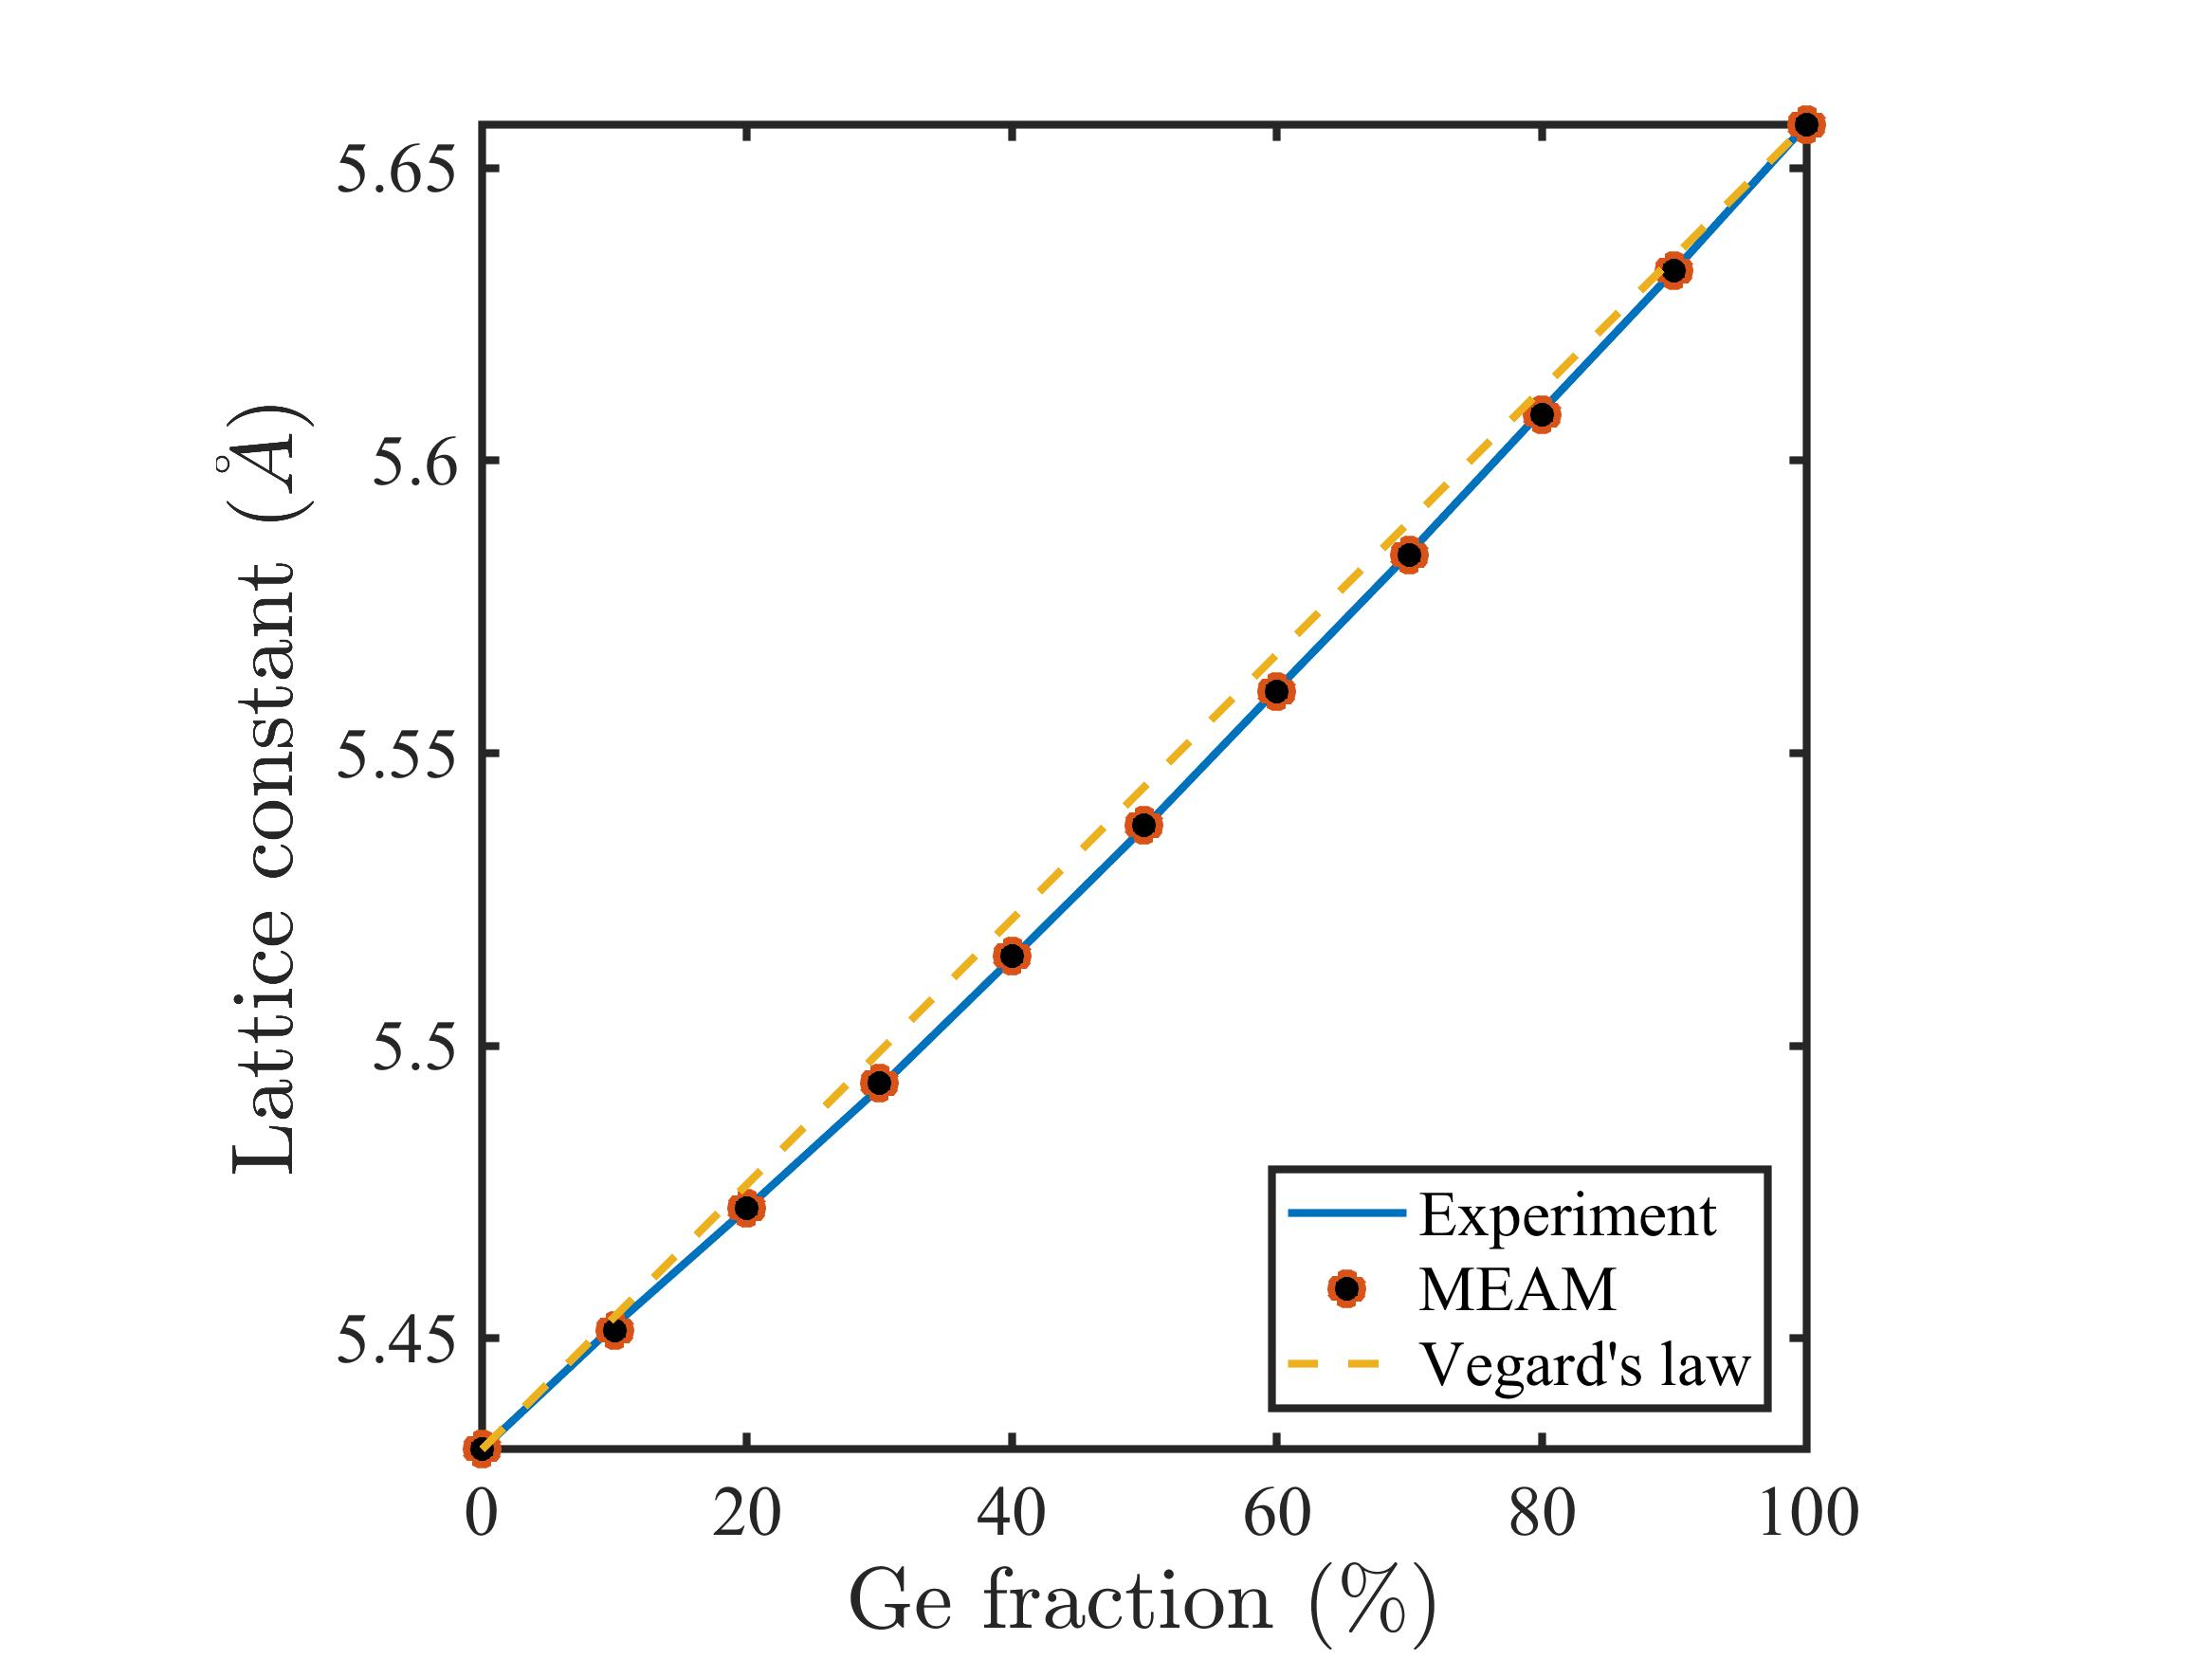
\includegraphics[trim = 0 0 0 2cm, clip, width=.5\linewidth]{Figures/latt_SiGe.jpg}
\caption{Lattice constants of $\rm Si_{1-x}Ge_x$.}
\label{fig:lattice_const}
\end{figure}

Fig. \ref{fig:lattice_const} shows that, with the parameters presented in Table \ref{tab:param}, the lattice constants fit to the experiments \cite{dismukes1964thermal} precisely. Note that the parameters for pure Si are adopted from \cite{ryu2009improved}. Those parameters are used in all the subsequent calculations.

\begin{table}[H]
% table caption is above the table
\caption{IMEAM model parameters for Si, Ge, and SiGe alloy potential (currently from Grochola 2010)}
\label{tab:param}       % Give a unique label
% For LaTeX tables use
\begin{tabular}{l  l   l   l   l   l   l   l   l   l   l   l   l    l   l   l }
\hline\noalign{\smallskip}
 Element  & $E_c$ & $r_e$ & $R_{\rm cut}$ & $B$ & $A$ & $\beta^(0)$ & $\beta^{(1)}$ & 
           $\beta^{(2)}$ & $\beta^{(3)}$ & $t^{(1)}$ & $t^{(2)}$ & $t^{(3)}$ & $C_{\rm max}$ & 
           $C_{\rm min}$ & $d$ \\
\noalign{\smallskip}\hline\noalign{\smallskip}\small
 Si       & 3.85 & 2.45 & 4.5 & 0.77 & 0.66 & 3.95 & 2.0 & 
          0.0 & 7.5 & 2.9 & 5.77 & -2.2 & 2.8 & 
           1.41 & 0.0 \\
 Ge     & 4.63 & 2.35 & 4.5 & 0.99 & 0.58 & 3.55 & 2.5 & 
           0.0 & 7.5 & 1.8 & 5.25 & -2.61 & 2.8 & 
          1.41 & 0.0 \\
 SiGe   & 4.23 & 5.529 & 4.5  & 0.88 &  &   &  & 
             &   &   &   &   & 2.8 & 
           1.41 & 0.0\\
\noalign{\smallskip}\hline
\end{tabular}
\end{table}


\begin{table}[H]
\centering
% table caption is above the table
\caption{Parameters for SiGe cross potential}
\label{tab:param_cross}       % Give a unique label
% For LaTeX tables use
\begin{tabular}{c c c c c c c c}
\hline\noalign{\smallskip}
$E_c(1,2)$ & $\Delta(1,2)$ & $\alpha(1,2)$ & $r_e(1,2)$ & $\rho_0(1)$ & $r_c$ & $C_{\rm max}$ &  $C_{\rm min}$ \\
\noalign{\smallskip}\hline\noalign{\smallskip}\small
 4.23 & 0.01 & 4.9716 & 2.3939 & 1.2719 & 4.5 & 2.80 & 1.41 \\
 \noalign{\smallskip}\hline
\end{tabular}
\end{table}
 }

It is worth mentioning that an attempt to reproduce the lattice constant fitting results of \cite{grochola2010modified} has been made. However, we found that the predicted value by their potential noticeably deviates from experimental findings, especially in the ${\rm x(Ge)=0.5}$ regime. Meanwhile,  three other critical issues in their work has been identified. I1) The correction functions to modify the radial distribution function of the liquid alloy developed in the paper is not implemented in LAMMPS. Although, it should not have significant effects on simulations of solid devices. ({\color{red}This issue needs to be removed})
I2) a mistake is identified in the parameter table for the r\_e column. 
I3) The claimed experimental lattice constant to fit to is $5.5285 {\rm \r{A}}$, but the actual experimental value is $5.5377 {\rm \r{A}}$. 
I4) How the lattice constant curve is obtained was not clearly stated. However, from the results, one can infer that the data should be obtained from finite temperature simulations, because otherwise the lattice constant of Si is not $5.431 {\rm \r{A}}$. Then  curves are shifted to match the lattice constant of Si with experimental value. 


\section{Melting temperature calculation {\color{red} LIVIA}}
\label{sec:melting_temperature}

%
Previous numerical studies with the SW potential  [cite SW1985, 1992] exhibit reasonable behavior for modeling shear properties and nucleation in silicon nanowires when compared to {\it ab initio} calculations (\cite{godet2009evidence} \cite{pizzagalli2013new}). SW has also been extensively used for dislocation nucleation in silicon for its success in predicting various mechanical and thermal properties of silicon.  However, it has been shown that SW cannot accurately predict the melting temperature of Ge \cite{ryu2008comparison}, overestimating it by approx. 1600K. {\color{red} did you calculate this? which method?} Thus, the melting temperatures of different compositions for $\rm Si_{1-x} Ge_x$ are expected to be significantly overestimated as well, suggesting that numerical predictions with the SW potential in the $900-1100$K regime are unreliable. 

%
%MEAM has demonstrated correct behaviors for the brittle-to-ductile transition of silicon, for example in \cite{kang2007brittle,kang2010size}). \cite{kang2007brittle} also presents a systematic performance comparison between SW and MEAM with respect to brittle-ductile transition behavior of silicon.  
%Minor changes have been proposed along the way of developing MEAM. These include changes in the form of the angularly dependent electron density term to make them orthogonal,[11], different ways to sum the partial electron density terms[12] and changes to the original screening functions to remove discontinuity[13].  There have been similar attempts for embedded atom method (EAM), which has been applied by {Glue Model [3], Finnis-Sinclair [4] or Volter-Chen [5] type CPL 2010} to model material properties over a large range of phase space.  

Calculating the melting temperature of semiconductor alloys is a challenging task due to the solubility of Si and Ge. To our knowledge, there exist no such systematic work presented in the literature. Although the focus of this study is not the fine tuning of the melting point ($T_m$) for specific applications, we attempt to calculate $T_m$ with as more confidence as possible. We used free energy calculation (FE) \cite{ryu2008comparison}  to verify the melting point of pure Si and Ge. We then applied both nested sampling (NS) and the two-phase co-existence (2P) methods to estimate the melting temperature at x(Ge)=0.25, 0.5, and 0.75. Nested Sampling is a recently developed free energy sampling method which does not require a prior knowledge of the alloy structure (CITE).

Table \ref{fig:tm} shows that $T_m$ of all compositions are captured within a reasonable range. The melting temperatures for both pure Si and Ge are precisely calculated with both 2P and FE methods. For the alloys, the two-phase coexisting method always converges to the solidus temperature. Similarly, NS calculation underestimates the melting by $\rm 200\,K$, which is possibly due to under-sampling of the phase space due to the cell size limitation. ({\color{red}This is very eye-catching and the reviewer may criticize. NS data may be moved to appendix.})

\begin{table}[H]
\centering
\caption{Melting temperature (error bar ?K) Exp, \cite{johnson1954some}; Tersoff. \cite{tersoff1988empirical},\cite{cook1993comparison}}
\label{tab:tm}
\begin{tabular}{lllllll}
\hline
Tm   (K)& x=0 & x=25 & x=50 & x=75 & x=100 &  \\ \hline
MEAM  (2P)   & 1644$\sim$1665    & 1505$\sim$1515      & 1386$\sim$1404      & 1241$\sim$1263    &  1194$\sim$ 1204 \\ 
MEAM  (NS)   & 1650   &  1450    &  1225    &  975  & 1180  \\
MEAM  (FE)   & 1640   &          &          &         & 1213  \\
SW      &   1694  &  --    &   --  &  --    &  2898 \\ 
Tersoff &  $\sim$3000K   &   --   &   --    &    --  &  $?$1874  \\ 
Exp     &  1685  &  1640(L), 1517(S)    & 1546(L),1381(S)   & 1402(L), 1279(S)     & 1210 \\ \hline
\end{tabular}
\end{table}

\section{Energy barrier for vacancy migration  {\color{red} Xiaohan}}
\label{sec:vacancy}
Vacancy diffusion is considered as the main mechanism that cause some serious mechanical or electrical damages. For example,  sessile dislocation loops such as Frank-Partials in SiGe are normally nucleated through the accumulation of vacancies. The aggregation of large number of vacancies can also bring about electrical short-cuts. Thus, accurately predicting the diffusivity of vacancy migrations is critical. In this last section, we use string method to quantify the energy barrier of a single vacancy migration, and compare it to some {\it ab-inito} results found in the literature [CITE Si. 0.1 N. Bernstein and E. Kaxiras, Phys. Rev. B 56, 10 488 1997] 
and [CITE 0.3 M. Tang, L. Colombo, J. Zhu, and T. Diaz De La Rubia, Phys. Rev. B 55, 14 279 1997.] [Ge. 0.4 eV. Negatively charged. ] Note that the migration energy barrier itself cannot give the diffusive rate without the prefactor which can be obtained through a large number of MD simulations [CITE PNAS2011]. 

\begin{figure}[H]
\centering
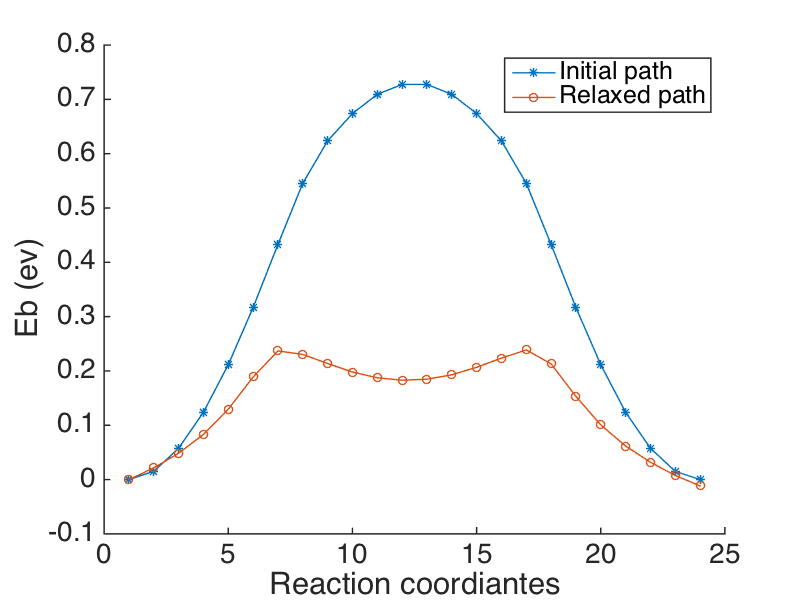
\includegraphics[width=.5\linewidth]{Figures/Eb_migration.png}
\caption{Energy barrier for migration of a vacancy in ${\rm Si_50Ge_50}$.}
\label{fig:Eb_migration}
\end{figure}

Fig. \ref{fig:Eb_migration} and \ref{fig:stateABS} show the minimum energy path (MEP) and the state A, B and saddle configurations along MEP. The initial straight path is relaxed and a middle saddle point is reached. The estimated energy barrier is 0.36 eV. 

\begin{figure}[H]
\centering
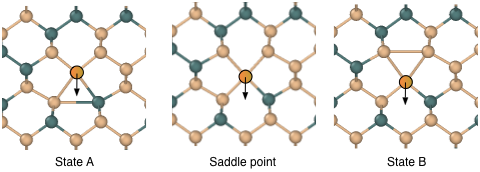
\includegraphics[width=.85\linewidth]{Figures/stateABS.png}
\caption{Configurations on MEP for vacancy migration in ${\rm Si_{0.75} Ge_{0.25} }$ system, induced by a diffusive Si (yellow) atom. Ge atoms are colored with blue.}
\label{fig:stateABS}
\end{figure}

\section{Elastic constants}
We first calculate the elastic constants given by the potential, as shown in Fig. \ref{fig:elastic_constants}

\begin{figure}[H]
\centering
% \subfigure[$C_{11}$] 
% {
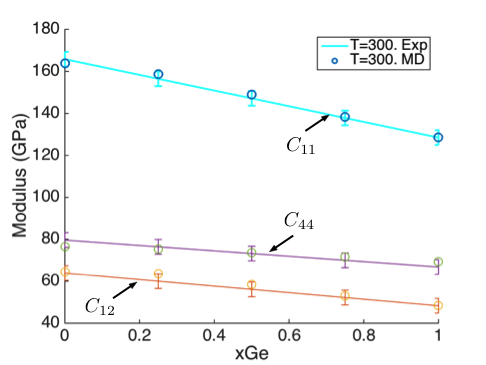
\includegraphics[width=.55\linewidth]{Figures/C11_12_44.png}
% }\hfill
% \subfigure[$C_{12}$] 
% {
% 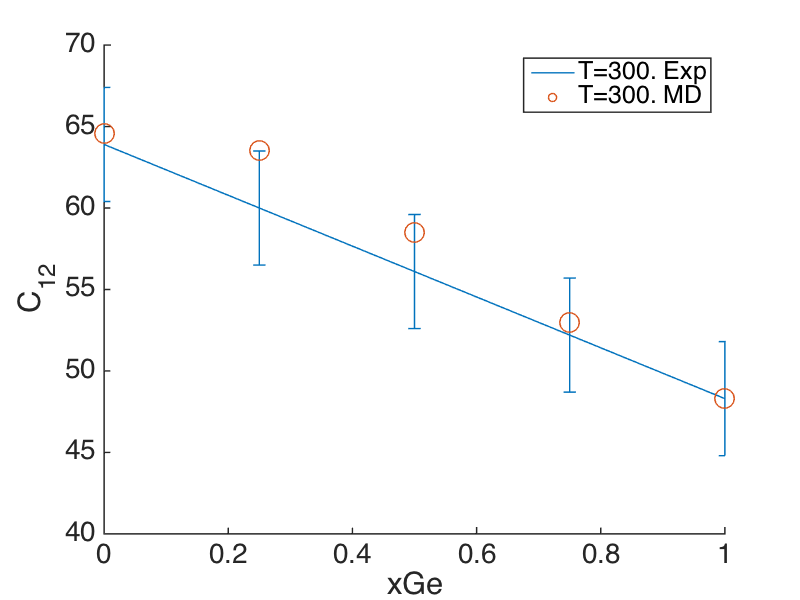
\includegraphics[width=.315\linewidth]{Figures/C12.png}
% }\hfill
% \subfigure[$C_{44}$] 
% {
% 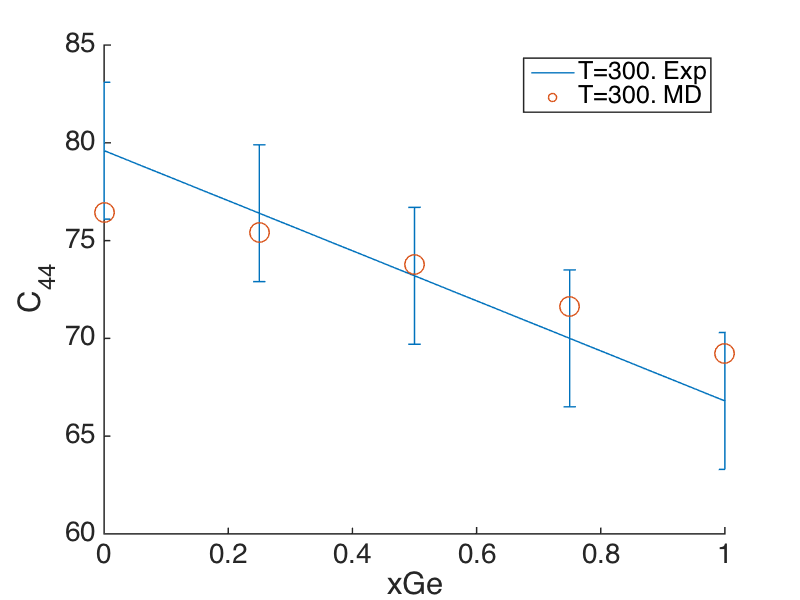
\includegraphics[width=.315\linewidth]{Figures/C44.png}
% }
\caption{$C_{11}$, $C_{12}$ and $C_{44}$ of ${\rm 300\,K}$  predicted by MEAM developed in this work.}
\label{fig:elastic_constants}
\end{figure}

Although homogeneous dislocation nucleation in bulk requires significantly larger energy and hardly observed in experiments, the simplified shear stress strain relationship from a bulk system reveals the fundamental strength and load capacity. Studying the finite temperature stress strain relationship help examine the difference in elastoplastic response between two potentials. 

Fig. \ref{fig:sscurve} shows the x-y shear stress and strain relationship at different temperatures. It is clearly observed that SW leads to earlier structural instabilities at elevated temperatures, compared to MEAM potential. At low temperature regime, the two potentials are satisfactorily consistent. The calculation demonstrates that SW-SiGe at high temperature seriously overestimates the bond-strength, which is consistent with the finding that the melting temperature given by SW is significantly higher than the experiments.

\begin{figure}[H]
\subfigure[x(Ge)=25]
{
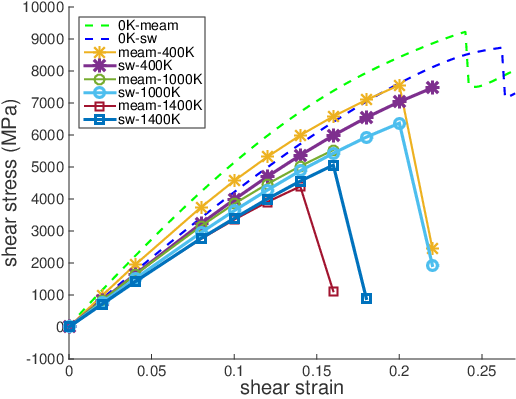
\includegraphics[width=.5\linewidth]{Figures/sscurve_x25.png}
}\hfill
\subfigure[x(Ge)=50]
{
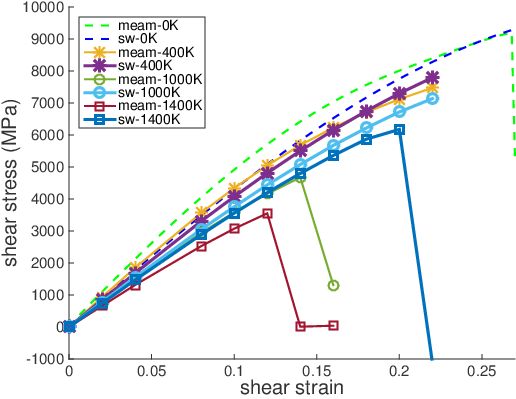
\includegraphics[width=.5\linewidth]{Figures/sscurve_x50.png}
}
\caption{Stress strain curve for ${\rm Si_50Ge_50}$ at different temperature. A comparison between SW-SiGe and MEAM developed by this work.}
\label{fig:sscurve}
\end{figure}

\section{Energy barrier for dislocation nucleation {\color{red} Xiaohan}} \label{sec:nucleation}
In this section, we show an application of the new potential in the field of dislocation nucleation. In reality of semiconductor fabrications, dislocations usually nucleate from a free surface or phase boundary, homogeneous nucleation is practically unlikely. In this section, we perform energy barrier calculations with both the improved MEAM potential and SW. The geometry considered is a thin film of which the free surface is perturbed by a rectangular pit of a few atomic layers. Such a geometry is motivated by practical semiconductor devices, e.g., \cite{grydlik2012misfit}, where a Si$(001)$ template patterns with an array of pits of $(111)$ side facets. Further more, having the pit structure is a way to mimic a roughened surface morphology that forms during SiGe thin film annealing. We refer to [cite zhang, cai] for detailed discussion.

%\begin{figure}[H]
%\centering
%\includegraphics[width=.5\linewidth]{/Users/x/Planet/Works/SU-2015-samsung/2015-nucleate/Graphics-Si-NEB/md-tf-pit/sscurve-pit.png}
%\caption{Molecular dynamics simulations of stress and strain relationship for thin film and surface pit structures (compression applied in $[110]$ direction).}
%\label{fig:sscurve-pit}
%\end{figure}

Fig. \ref{fig:neb-sige} shows the NEB calculations with both MEAM and SW potential. It is observed that the results from both potentials are consistent. The NEB calculations show that the energy barrier for nucleating a dislocation in such a surface pit thin film will vanish after the compressive strain reaches $6\%$ strain. In practice, the semiconductor system cannot sustain such a large strain energy. Some other failure mode will precede. See cite[zhang, cai]. However, it is not our intention here to identify or discover what nucleation mechanism should come at first place during the deposition process, which has been a puzzling problem for decades. The numerical calculation shows that the 0K energy barrier of the improved MEAM potential is ``at least'' as accurate as SW potential. And note that SW potential has been the dominant potential applied to study related problems. 

\begin{figure}[H]
\centering
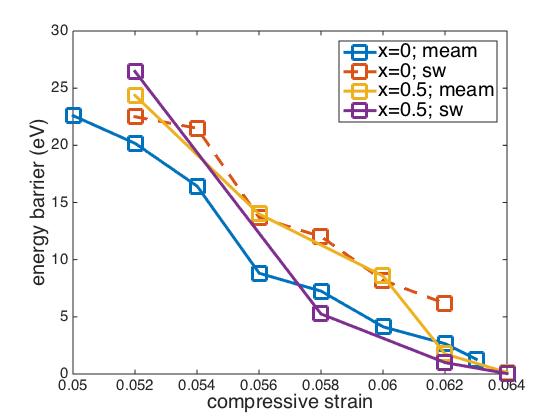
\includegraphics[width=.5\linewidth]{Figures/neb_plot_sige.png}
\caption{State A and state B for energy barrier calculations.}
\label{fig:energy_barrier}
\end{figure}



\section{Numerical methods}
%\appendix
\subsection{Molecular Dynamics (two-phase coexistence method, stress strain calculation)}\label{sec:md}
We used the Lammps package (\cite{plimpton1995fast}) for all finite temperature Molecular Dynamics simulations.  Verlet algorithm for time integration was adopted for time steps of $0.5 {\rm fs}$. We applied Nos{\'e}-Hoover thermostat in the NVT ensemble to maintain the system at the desired temperature levels, from $400{\rm K}$ to $1400 {\rm K}$. The bulk simulation for the stress-strain curves included 14400 atoms. The simulation cell of the thin film had a dimension of $192 {\rm \r{A}} (x)$, $192{\rm \r{A}} (y)$ and $214{\rm \r{A}} (z)$ and contained $3.6\times 10^5$ atoms. The free surface of the thin film was created by expanding the simulation box by $1.2$ in the $z$ direction. Periodic boundary conditions were applied in both the $x$ and $y$ directions. A surface pit was created on the $(001)$ surface with a depth of $21.4{\rm \r{A}}$. A compressive strain was applied along the $[110]$ direction, at the strain rate of $2\times 10^8 \, s^{-1}$.  

Another popular potential choice is Tersoff which is preferred when modeling high temperature solid behaviors such as amorphous core shell nanowires [cite Shan]. However, it is widely known that the system described by Tersoff is over-stiff thus cannot have ductility behaviors, which is clearly different from the experiments [{\color{red} CITE NIX students}]. {\color{red} this section on Tersoff should go somewhere else. maybe intro or where the SW is discussed?}

\subsection{A modified string method for energy barrier calculation}\label{sec:neb}
A modified string method was applied to find saddle points and the associated Minimum Energy Path (MEP). The method takes a chain of atomic configurations as input and performs constrained relaxation on each node until it finds the MEP while maintaining equal spacing to neighboring images. Thus, every configuration is allowed to relax independently. This is different from the traditional string method where constraints are applied during the relaxation. After a predetermined number of relaxation steps, the path is reparametrized between the two endpoints using linear interpolation between each of the existing configurations. The location of these new interpolated configurations is such that the path is equally divided with a constant distance (in phase space) between each neighboring pair of configurations.  This new algorithm runs efficiently in parallel mode and overcomes several difficulties occurred in classical string methods such as instability and poor discretization when applied to high-stress conditions and/or to semiconductors.

The simulation cell for all NEB calculations had a size of $81.4{\rm \r{A}} (x)$, $81.4{\rm \r{A}} (y)$ and $114{\rm \r{A}} (z)$, containing $14400$ atoms. The free surface of the thin film was created by expanding the simulation box by $20\%$ in the $z$ direction. Periodic boundary conditions were applied in both $x$ and $y$ directions. 

A crucial part of the Minimum Energy Path analysis is to prepare an energetically stable, dislocation-free reference state with and without the surface irregularity. We noticed that the dangling atomic bonds on the $(001)$ surface caused major energy disturbances to the calculations due to random surface reconstructions. The free surface atoms -- each having $3$ dangling bonds -- tend to randomly form clusters with neighboring atoms and release bonding energy, thus yielding either random or non-convergent result. To eliminate these disturbing factors, we formed dimer bonds in the $[110]$ direction by manually displacing surface atoms towards each other, as shown in Fig. \ref{fig:reconstruction}(b). The system is then relaxed to a local energy minimum which has a much lower energy than the initial structure.  We found that such a systematic surface reconstruction is indispensable during energy barrier calculations, as without such preparations, the numerical results are not reproducible. We used the reconstructed state as the starting point of energy barrier calculation and MD simulations. 

% \begin{figure}[H]
% \subfigure[before surface reconstruction]
% {
% \includegraphics[ width=.45\linewidth, height=.35\linewidth]{../Graphics/Si-recons-illus-2_converted.png}
% }\hfill
% \subfigure[dimer-constructed configuration]
% {
% \includegraphics[ width=.45\linewidth, height=.35\linewidth]{../Graphics/Si-recons-illus_converted.png}
% }
% \caption{Displacing surface atoms to reconstruct dimers out of dangling bonds. Yellow atoms are on $(001)$ surface.}
% \label{fig:reconstruction}
% \end{figure}

\subsection{Nested Sampling Method}\label{sec:ns}

Nested sampling (NS) is a Bayesian statistical method~[\cite{bib:skilling,bib:skilling2}] adapted to explore the atomic phase space~[\cite{our_NS_paper}].
The NS algorithm does not require prior knowledge of the phases or phase transitions and takes only the potential energy function together with the desired pressure and temperature ranges as inputs. 
Moreover, the direct output of the simulation is the partition function as an explicit function of its natural variables, so calculating different thermodynamic observables, such as compressibility or heat capacity, is straightforward.
NS has been applied to study clusters and the hard-sphere model ~[\cite{our_NSHS_paper, diffns,Frenkel_NS}], and it has been shown that the NS algorithm enables the automated calculation of the complete pressure-temperature-composition phase diagram~[\cite{pt_phase_dias_ns,pymatnest_paper}].

The nested sampling calculations in the current work were performed using the pymatnest program package [\cite{pymatnest}] as presented in~\cite{pt_phase_dias_ns}. The simulations were run at constant pressure of , and the simulation cell of variable shape and size contained 64 atoms. 
The initial configurations were generated randomly. 
New samples were generated with performing Hamiltonian Monte Carlo~\cite{pymatnest_paper} (all-atom) moves, and changing the volume and the shape of the cell by shear and stretch moves, introducing swap moves in the bicomponent systems.
Overall 12000 steps were performed at every iteration with ratio 1:4:2:2, respectively, and the number of walkers were set to be 800.

The calculations may include x =0, 0.25, 0.5, 0.75, 1. We can compare pure Si and pure Ge with previous works. Also, please clarify the ``definition'' of melting point in your calculation. Ideally, for each x, we should have both SW and meam.



\section{Conclusions and Future Works}
\label{sec:conclusions}

We developed a Modified Embedded Atom Method potential for atomistic simulations with $\rm Si_xGe_{1-x}$ alloys. The potential is the first MEAM potential that demonstrates accuracy in both thermal and mechanical properties. We point out that SW predicts twice as high melting temperature as the experiments which makes it inappropriate to be used for under temperature conditions. The elastoplastic behavior of MEAM potential is close to SW characterized by the dislocation nucleation energy barrier. 


\section{Acknowledgement}
This work is supported by Samsung SSI (X.Z) and  supported by the U.S. Department of Energy, Office of Basic Energy Sciences, Division of Materials Sciences and Engineering under Award No. DE-SC0010412 (W.C.).
%

\iffalse
\section{Tech details}

\begin{enumerate}
\item  pure silicon, 0K, SW underestimates shear modulus: C44 is less than experiment by 30\%., C12 is larger by 25~30\%.  \\

e.g., \\
Molecular dynamic calculation of elastic constants of silicon, 1986
Comparative study of silicon empirical interatomic potentials, 1992

\item  The experimental value for silicon shear modulus varies from 50.9 GPa to 79.4 GPa. According to NSM webpage it is 51 GPa. 
http://www.ioffe.ru/SVA/NSM/Semicond/SiGe/mechanic.html 

\item The 0K stress strain curves with the new potential. The shear modulus for pure Si is 56 GPa (meam) and 42 GPa (sw). The system I tested is [1-2 1] x [111] x[10-1]. shear along yz direction. For Ge, SW and MEAM are consistent. With increasing Ge concentration, the difference between SW and MEAM becomes smaller.

\item 0K stress strain curve of SW: mc2:/home/xzhang11/Planet/Libs/MD++.svn/runs/ho-sige-DN, scripts: mc2:/home/xzhang11/Planet/Libs/MD++.svn/scripts/work/SiGeHomo-sworig/ss\_sige.tcl) \\
0K stress strain curve of MEAM:  mc2:/home/xzhang11/Planet/Libs/MD++.svn/runs/ho-sige-DN-meam, scripts: mc2:/home/xzhang11/Planet/Libs/MD++.svn/scripts/work/SiGeHomo-sworig/ss\_sige.tcl) \\
matlab$>>$plot(strain(:,2),stress(:,6))
\end{enumerate} 
\fi 
\bibliography{blackout}

\end{document}